%
% CHAPTER Versuch 4
%
\chapter{Pixelfehler}
Betrachtung von Pixelfehlern und Anwenden der Kalibrierung mit Dunkel und Weißbild.
\label{chap:Pixelfehler}

\section{Fragestellung, Messprinzip, Aufbau, Messmittel}
Je nach Qualität des Bildsensors gibt es durch den Fertigungsprozess funktionsuntüchtige Pixel. Bei diesen Pixeln handelt es sich um Deadpixel, Stuck oder Hotpixel. Bei Hotpixeln handelt es sich um Bildpunkte, welche nach längerer Belichtungszeit in die Sättigung gehen. Stuckpixel sind Pixel, welche sich stets auf ihrem Maximalwert befinden. Stuck und Hotpixel lassen sich am einfachsten auf dem Dunkelbild erkennen. Deadpixel sind Pixel, die quasi tot sind. Dies bedeutet sie sind permanent auf dem Wert null liefern also immer Schwarz. Diese Art von Pixelfehler können nicht durch eine Kalibrierung behoben werden. Deshalb wird in diesem Versuch auch nichts unternommen, um diesen Fehler zu beheben. Diese Bildfehler können jedoch durch Interpolation behoben werden.
Um unser Testbild \ref{img:Grauwertkeil} zu korrigieren, gilt es nun den durch das Dunkelbild berechnete Offset der Pixel zu entfernen. Desweiteren wird das Bild noch durch das in Versuch drei (Kapitel \ref{chap:VERSUCH_3}) berechnete und normierte Weissbild geteilt um die Sensitivität anzupassen.
Im Anschluss wird uns ein Pythonskript \ref{lst:Graustufen} die Differenz der einzelnen Bereiche zwischen dem original Graukeilbild und dem korrigierten Graukeilbild berechnen. Hierzu wird das Bild zunächst in die einzelnen Graustufen zerlegt. Im Anschluss wird der durchschnittliche Helligkeitswert dieser Graustufe, wie auch die Standartabweichung, was dem Rauschen der Pixel entspricht, berechnet. 
Beim Vergleichen dieser Werte sollte sich eine Besserung des Bildes feststellen lassen. Die Verbesserung des Rauschverhaltens sollte in der Standartabweichung ersichtlich werden. Das heißt es wird erwartet, dass der Betrag der Standartabweichung sinkt. 
\label{chap:VERSUCH_4_FRAGESTELLUNG}

\section{Messwerte}
\begin{figure}[H]
\centering
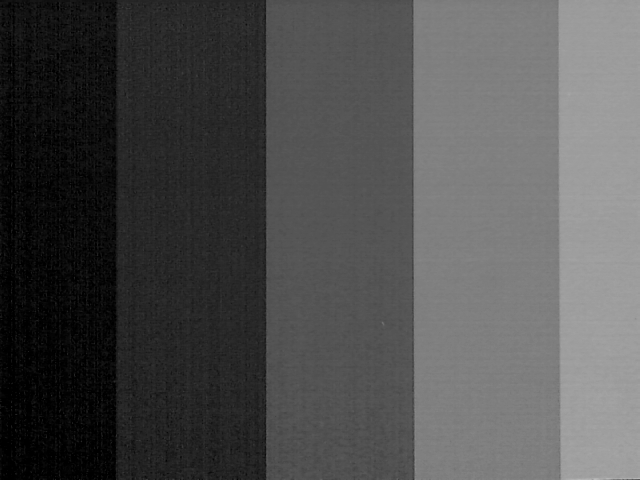
\includegraphics[width=150mm]{graustufen_korrigiert.png}
\caption{Graukeil kalibriert.}
\label{img:Graukeil_korrigiert}
\end{figure}


\begin{figure}[H]
\centering
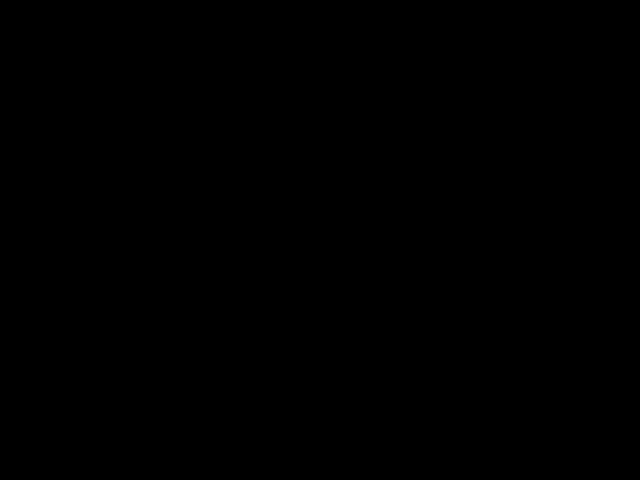
\includegraphics[width=150mm]{dunkelbild_1.png}
\caption{Dunkelbild}
\label{img:Dunkelbild_normal}
\end{figure}


\begin{figure}[H]
\centering
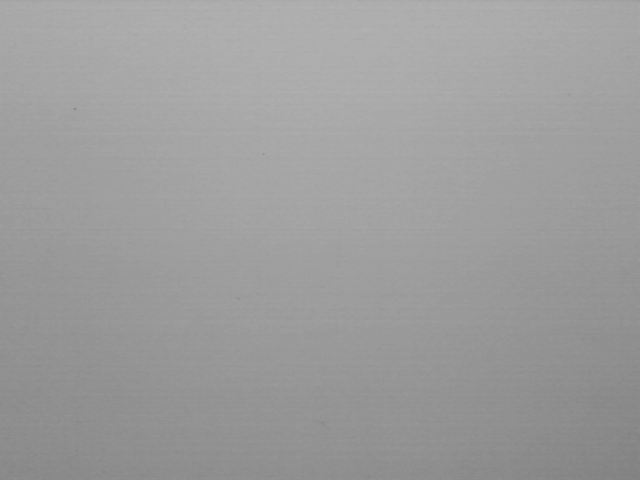
\includegraphics[width=150mm]{weissbild_1.png}
\caption{Weißbild}
\label{img:Weissbild_normal}
\end{figure}

\label{chap:VERSUCH_4_MESSWERTE}

\section{Auswertung und Interpretation}
Bei genauerer Betrachtung des Dunkelbildes \ref{img:Dunkelbild_normal} fallen keine weißen Punkte ins Auge. Es sind also keine Hot oder Stuckpixel zu erkennen. Es finden sich auch keine Deadpixel in dem Weißbild wieder. Die hier gefundenen schwarzen Punkte sind lediglich durch Kontrastmaximierung schwarz und somit keine Deadpixel. Weiter lassen sich in diesem Fall auch keine Deadpixel sicher detektieren, da die Weiße Fläche nicht völlig homogen war.
Zum korrigieren unseres Graukeilbildes wird zuerst das Dunkelbild abgezogen und anschließend durch das Weissbild dividiert. Die Formel $y = a\cdot x+b$ erklärt dieses Vorgehen. $y$ ist der durch die Kamera gelieferte Pixelwert. Dieser berechnet sich aus dem tatsächlichen Wert $x$, der Sensitivität $a$ und dem Offset $b$. Durch Subtraktion des Offsets $b$, welcher uns das Dunkelbild liefert, und anschließender Division der Sensitivität $a$, welche uns das Weissbild liefert, erhalten wir die Formel: $x = \frac{y-b}{a}$ und somit den tatsächlichen Pixelwert.
Das im Pythonskript TODO REF berechnete neue Graustufenbild wird genau wie das Original in seine einzelnen Stufen zerlegt. Für diese Graustufen $(g1 - g5)$ werden jetzt jeweils Mittelwert und Standartabweichung berechnet \ref{tab:VGL-TAB}. Hierbei wird deutlich, dass durch die Korrektur eine deutliche verbesserung erzielt wurde. das Rauschen, sichtbar an der Standartabweichung, wurde um bis zu 79 \% verbessert.

In folgender Tabelle sind die Graustufen von g1 (Weiss) bis g5 (Schwarz) aufgelistet.
\begin{table}[H]
\centering
\begin{tabular}{c|ccccc}
Graustufe & Durchschnitt vorher & nachher & Stdabw vorher & nacher & Verbesserung in \% \\
\hline
g1 & 9.3699 & 9.2598 & 7.4903 & 7.1983 & 3.8981\\
g2 & 39.1486 &  38.6003 & 5.9921 & 4.5087 & 24.7560\\
g3 & 85.7785 & 83.8205& 6.9256 & 2.5537 & 63.1272\\
g4 & 126.9901 & 127.3212 & 8.8584 & 2.3224 & 73.7836\\
g5 & 152.3874 & 157.0740 & 9.1518 & 1.8588 & 79.6893\\

\end{tabular}
\label{tab:VGL-TAB}
\caption{Vergleich vor und nach Kalibrierung.}
\end{table}
Bei genauerer Betrachtung des Graukeilbildes fällt in der unteren rechten Ecke ein Fehler auf, welcher bei der Aufnahme des Bildes gemacht wurde. Der Grauwertkeil lag nicht so, dass er das gesamte Bild ausfüllte. Damit dieser Fehler keinen Einfluss auf den Durchschnittswert der weissen Graustufe hat, werden die untersten 20 Pixel ausgelassen, dies wird im Pythonskript \ref{lst:Graustufen} ersichtlich.
Die Werte der Tabelle, vor allem die letzte Spalte zeigt, dass der Aufwand in den vorhergehenden Teilaufgaben nicht vergebens war, das Rauschen wurde vor allem in den letzten drei Zeilen sehr effektiv beseitigt.
\label{chap:VERSUCH_4_AUSWERTUNG}